\documentclass[titlepage]{article}
\usepackage{polyglossia}
\usepackage{fontspec}
\setmainlanguage{russian}
\setmainfont{Times New Roman}
\usepackage{varwidth}
\usepackage{sectsty}
\usepackage{graphicx}
\usepackage[labelsep=endash]{caption}
\usepackage{geometry}
 \geometry{
 a4paper,
 left=20mm,
 top=20mm,
 }
\usepackage{fancyhdr}
\pagestyle{fancy}
\fancyhf{}
\renewcommand{\headrulewidth}{0pt}
\rhead{\thepage}
\usepackage{indentfirst}
\usepackage{floatrow}
\floatsetup[table]{capposition=top}
\graphicspath{ {images/} }
\sectionfont{\centering}
\renewcommand{\labelitemi}{\textendash}
\newcommand{\goal}[1]{\textit{Цель работы:} #1}
\begin{document}
\captionsetup[figure]{name={Рисунок}}
\begin{titlepage}
\begin{center}
\MakeUppercase{Харьковский национальный университет радиоэлектроники}

\vspace*{\fill}
Отчет

по лабораторной работе №1

по теме "Моделирование задач многокритериального принятия решений"

\end{center}
\vspace{20mm}
\hfill
\begin{varwidth}{\linewidth}
Выполнили\\
ст. гр. ПЗСм-17-3\\
Гранкина Валерия\\
Гройс Михаил\\
Карачевцев Кирилл\\
Савченко Дмитрий\\

Проверила\\
доц. Мазурова О. А.
\end{varwidth}
\vspace*{\fill}

\centering{Харьков 2018}
\end{titlepage}
\goal{приобрести навыки использования и программной реализации средств информационной подготовки задач многокритериального принятия решений. Познакомиться с методами описания многокритериальных альтернатив, разных шкал оценивания альтернатив по критериям, методов нормирования оценок по разным типам шкал.}
\section*{Описание физической модели БД}

Физическая модель базы данных состоит из шести таблиц:
\begin{itemize}
\item Alternative --- таблица, которая содержит возможные альтернативы;
\item Criterion --- таблица критериев;
\item Mark --- таблица возможных оценок для каждого критерия;
\item Vector --- таблица, связывающая оценки и альтернативы;
\item LPR --- таблица с личностями, которые принимают решения;
\item Result --- таблица результатов.

Детальное описание схемы представлено на рисунке \ref{fig:schema}.

\begin{figure}[h]
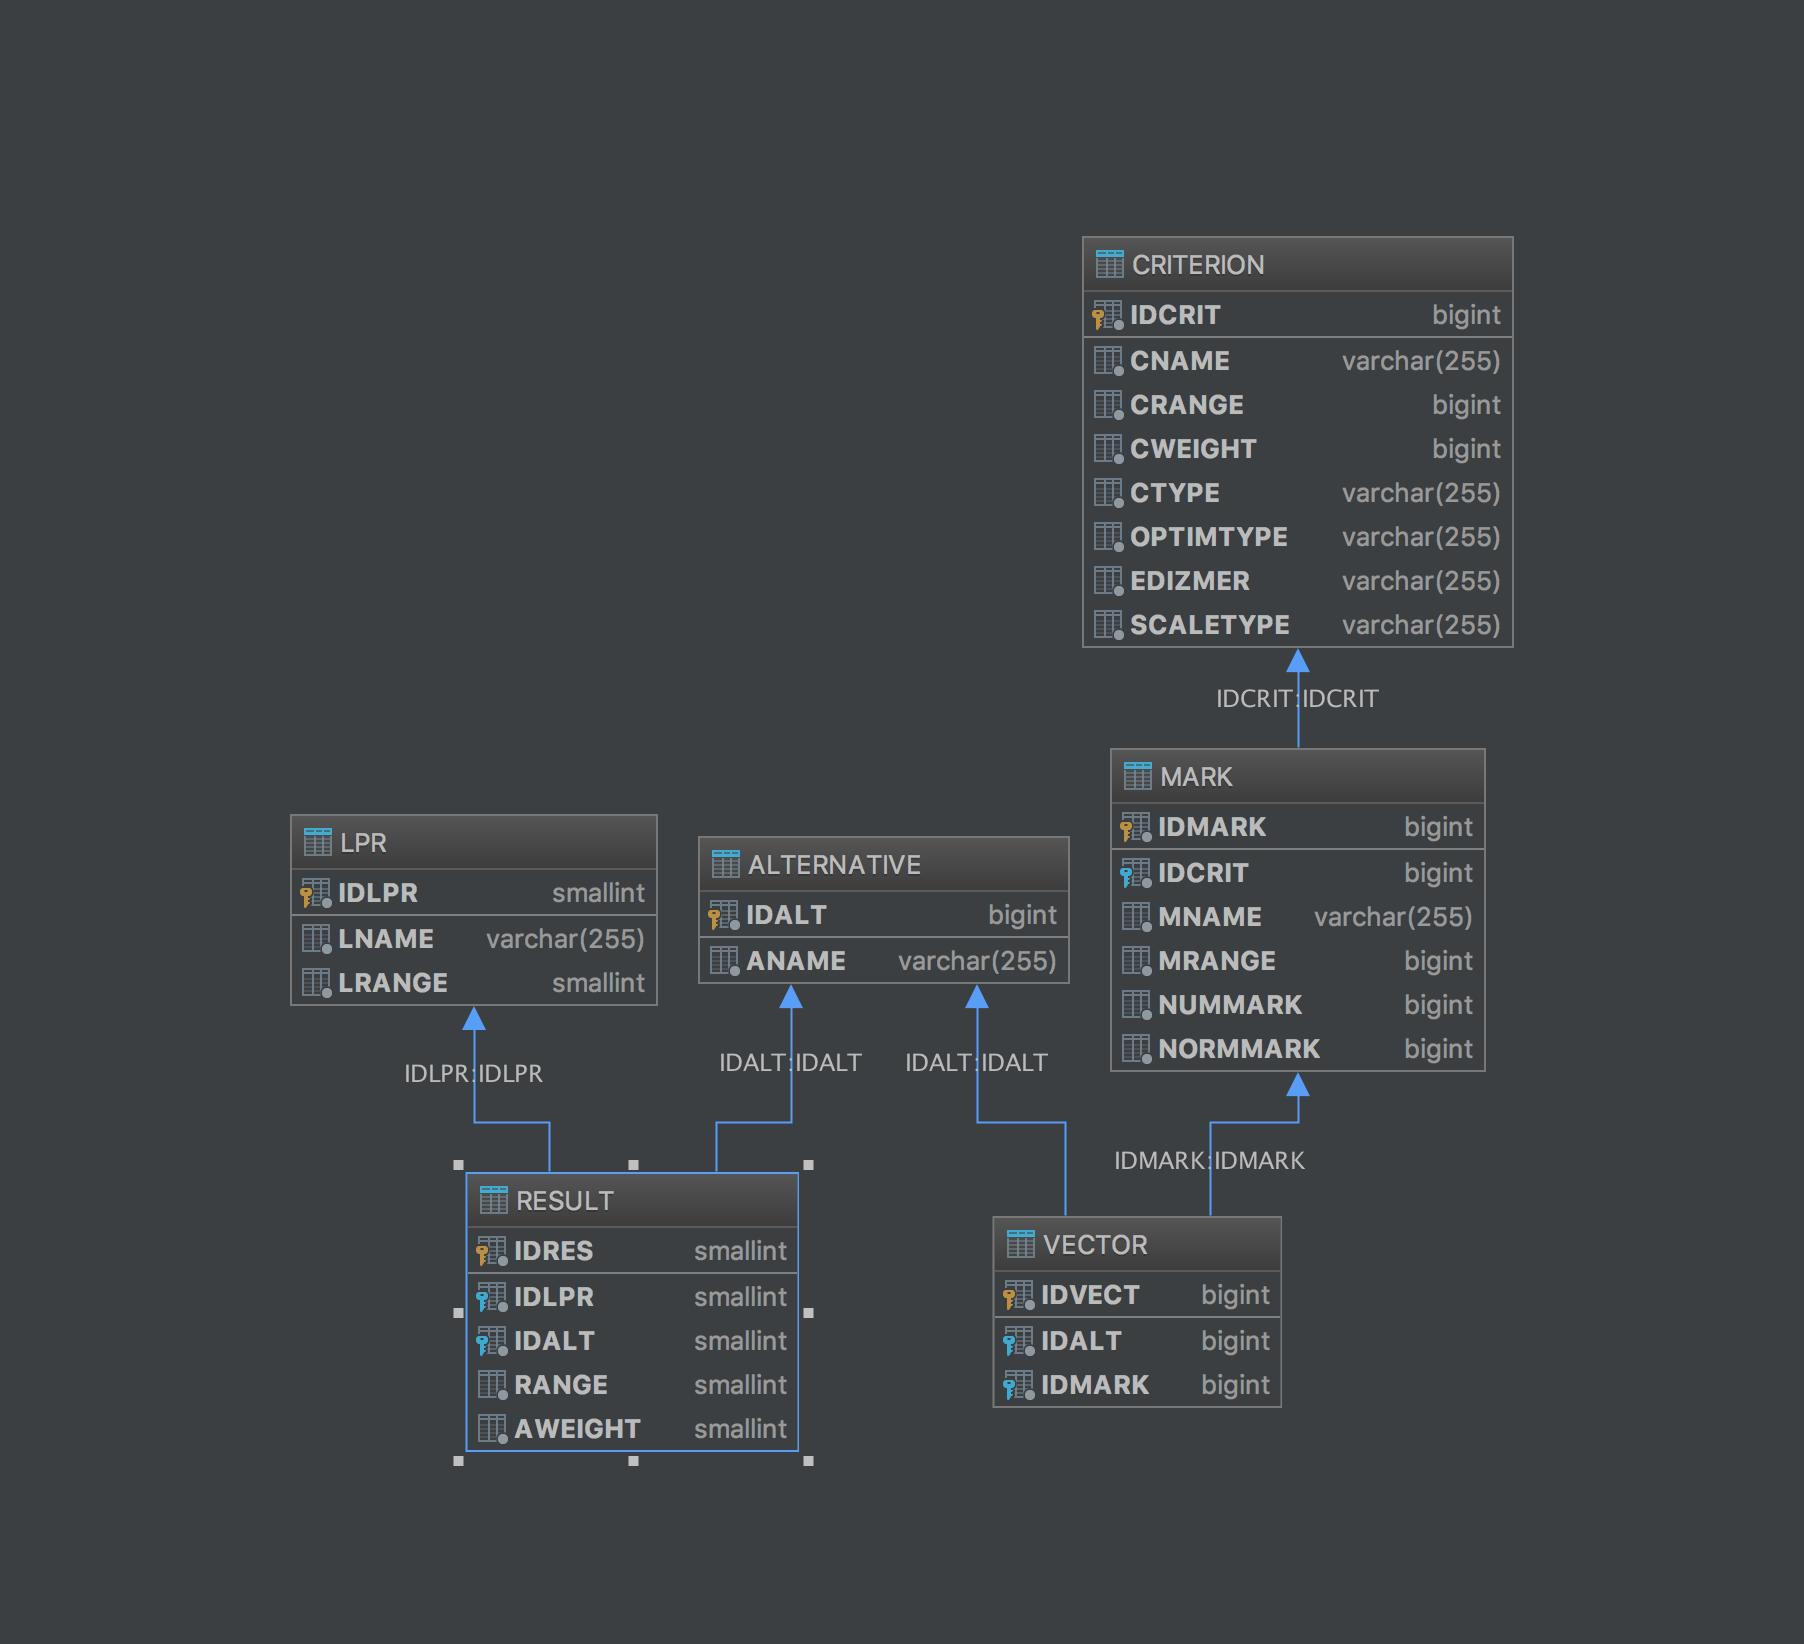
\includegraphics[scale=0.4]{schema}
\caption{Схема базы данных}
\label{fig:schema}
\end{figure}
\end{itemize}

\section*{Описание информационной модели принятия решений}

\begin{center}
Вариант №7

"Выбор ноутбука"
\end{center}

Информационная модель состоит в следующем:
\begin{itemize}
\item альтернативы для выбора:
\begin{enumerate}
\item HP 2017 15.6" Full-HD IPS UWVA Laptop;
\item Dell Latitude E7470 Business Ultrabook;
\item Apple MacBook Pro MF839LL/A;
\item Lenovo Yoga;
\item ASUS K501UW-AB78;
\end{enumerate}
\item критерии и оценки:
	\begin{enumerate}
		\item диагональ экрана (дюймы):
			\begin{enumerate}
			\item 13.5;
			\item 15.3;
			\item 17.1;
			\end{enumerate}
		\item вес (кг):
			\begin{enumerate}
				\item 1.29;
				\item 1.37;
				\item 1.25;
			\end{enumerate}
		\item батарея (часы):
			\begin{enumerate}
				\item 13;
				\item 10;
				\item 14.5;
			\end{enumerate}
		\item производитель:
			\begin{enumerate}
				\item Dell;
				\item Apple;
				\item Lenovo;
				\item Asus;
				\item HP;
			\end{enumerate}
		\item процессор:
			\begin{enumerate}
				\item Intel i5;
				\item Intel i7;
				\item Intel i3;
			\end{enumerate}
		\end{enumerate}
\item векторное описание альтернатив представлено в таблице \ref{tab:vector}.
\begin{table}[h]
\centering
\caption{Векторное описание альтернатив}
\label{tab:vector}
\begin{tabular}{|l c c c c c|}
\hline
\empty & Диагональ экрана & Вес & Батарея & Производитель & Процессор \\
\hline
HP 2017 15.6" Full-HD IPS UWVA Laptop & 13.3 & 1.37 & 13 & HP & Intel i5 \\
Dell Latitude E7470 Business Ultrabook & 13.5 & 1.29 & 14.5 & Dell & Intel i7 \\
Apple MacBook Pro MF839LL/A & 15.3 & 1.25 & 14.5 & Apple & Intel i3 \\
Lenovo Yoga & 17.1 & 1.25 & 10 & Lenovo & Intel i5 \\
ASUS K501UW-AB78 & 15.3 & 1.29 & 13 & Asus & Intel i5 \\
\hline
\end{tabular}
\end{table}
\end{itemize}

\section{Экранные формы}

Просмотр альтернатив представлен на рисунке \ref{fig:alternatives}.
\begin{figure}

\includegraphics[scale=0.4]{alternatives}
\caption{Альтернативы}
\label{fig:alternatives}
\end{figure}

Критерии, оценки и векторы представлены на рисунках \ref{fig:criteria}, \ref{fig:marks}, \ref{fig:vectors} соответственно.

\begin{figure}
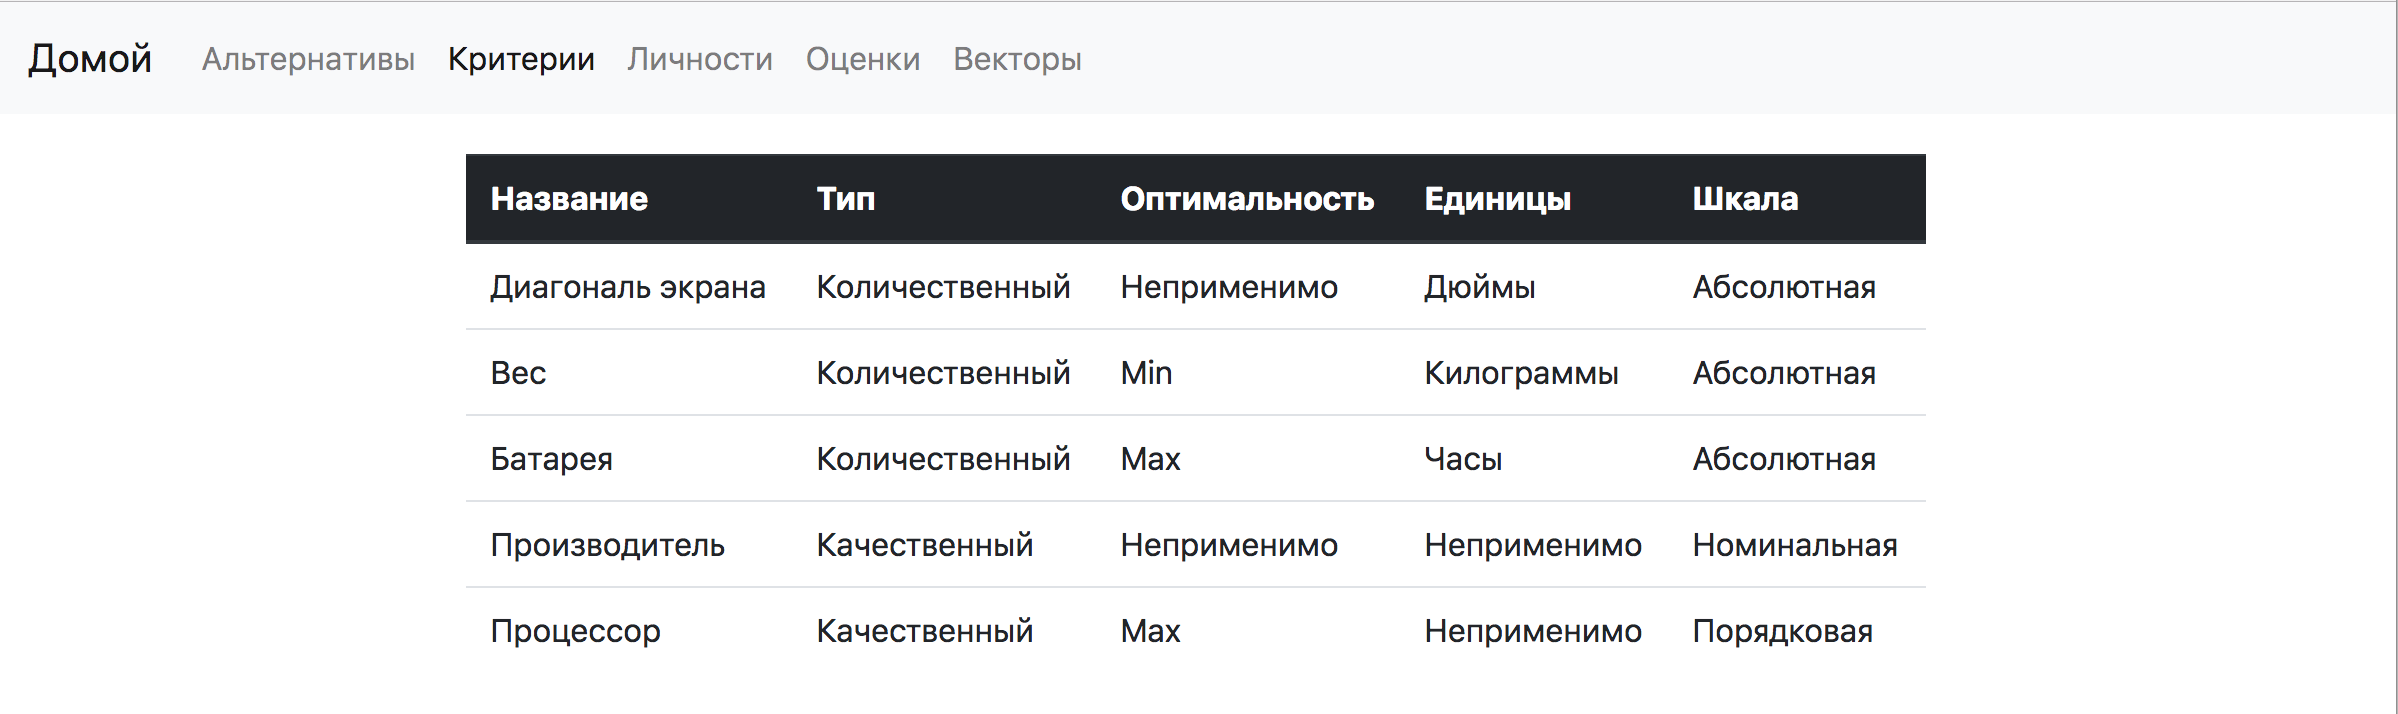
\includegraphics[scale=0.4]{criteria}
\caption{Критерии}
\label{fig:criteria}
\end{figure}

\begin{figure}
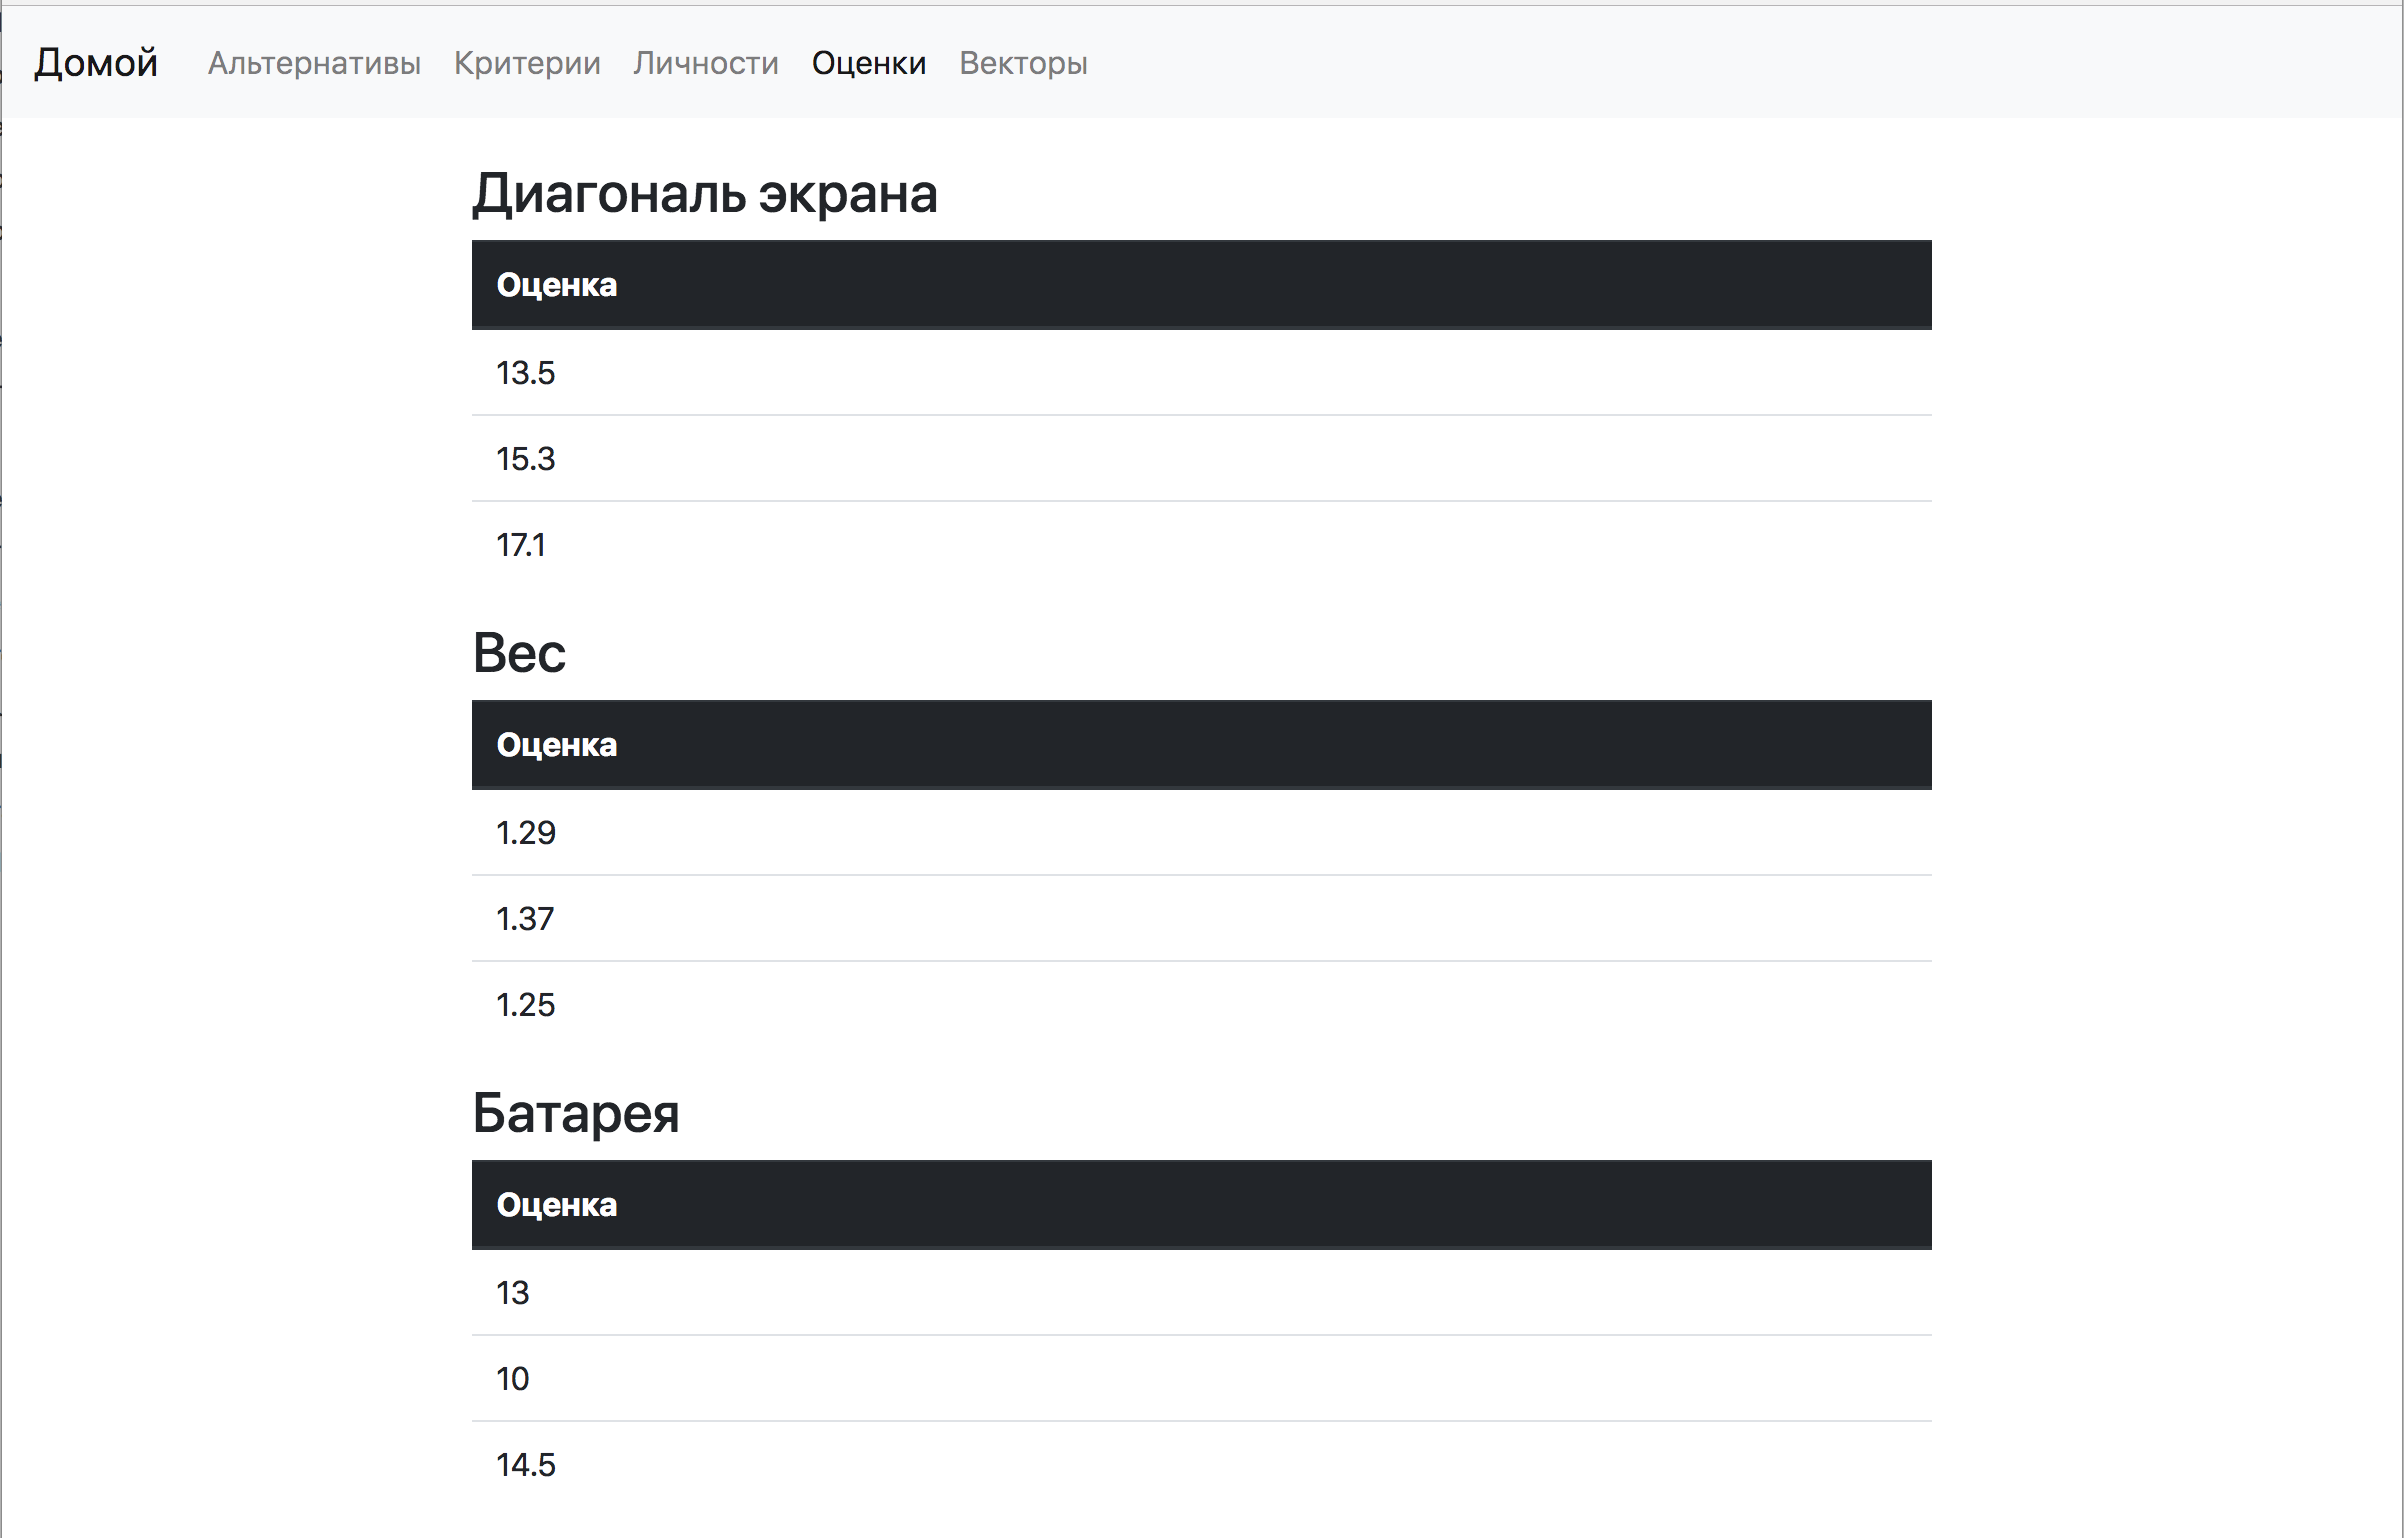
\includegraphics[scale=0.4]{marks}
\caption{Оценки}
\label{fig:marks}
\end{figure}

\begin{figure}
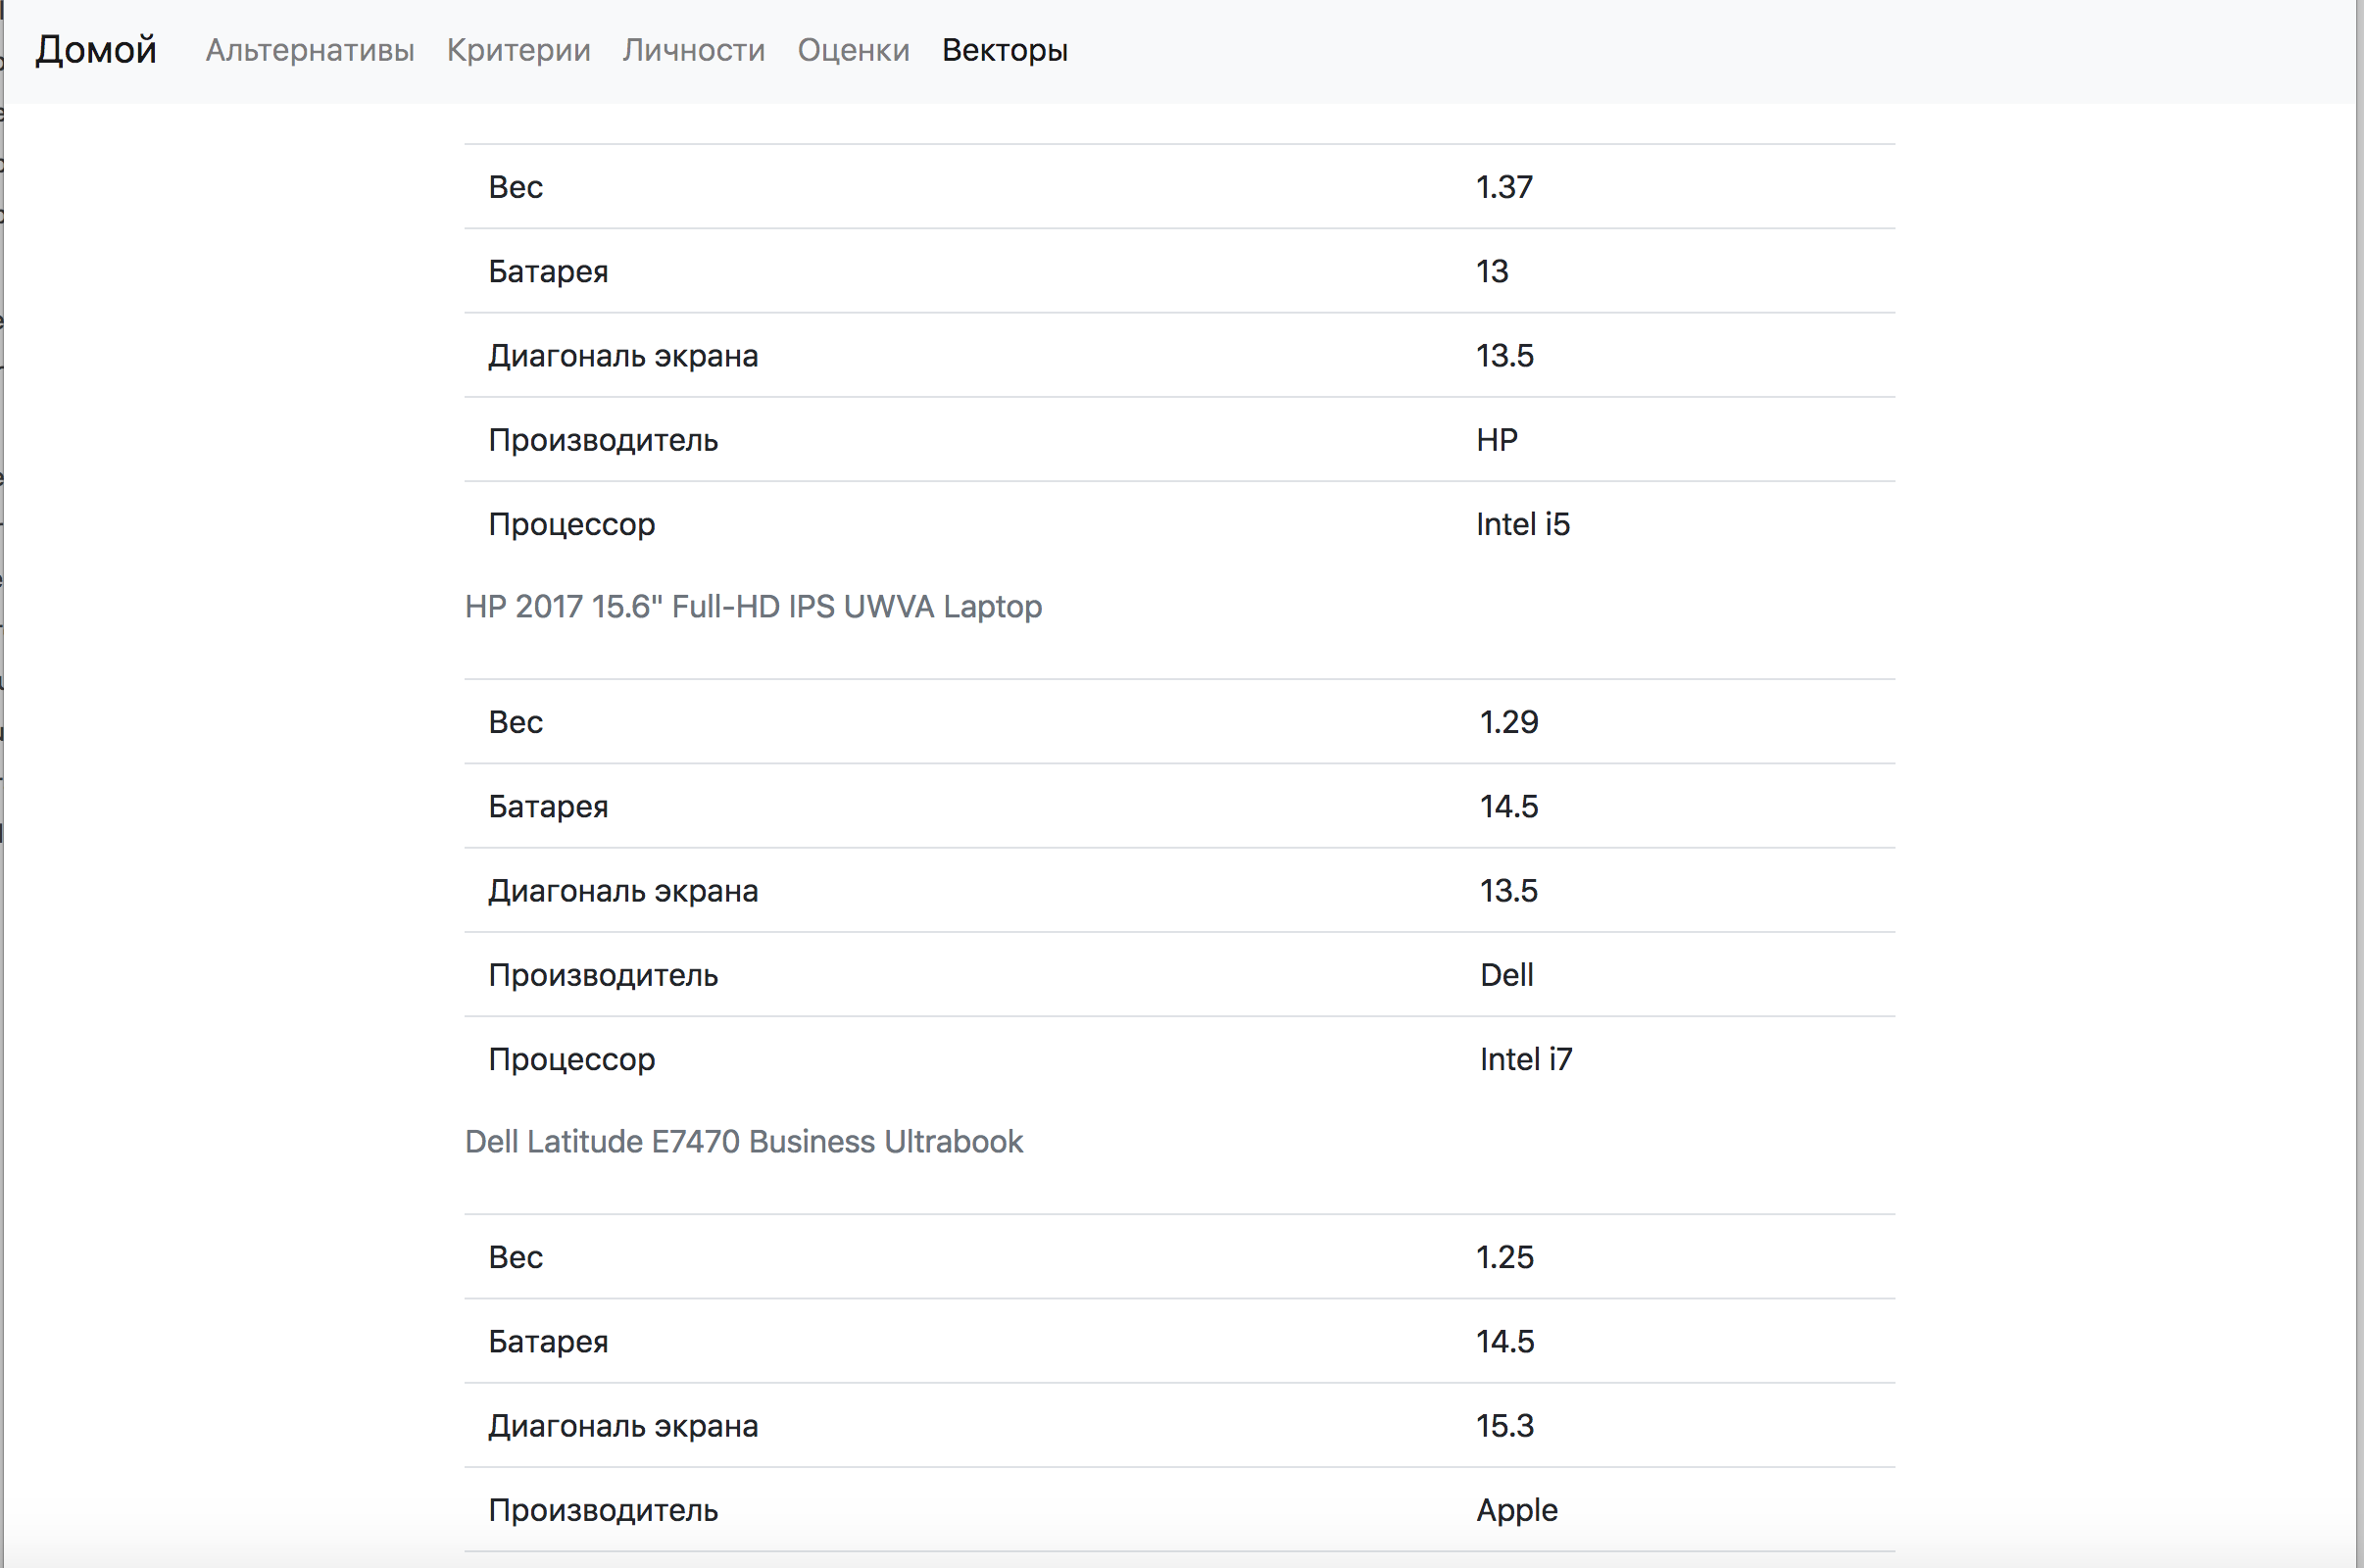
\includegraphics[scale=0.4]{vectors}
\caption{Вектор альтернатив}
\label{fig:vectors}
\end{figure}

\end{document}
